\begin{block}{Spatially Aggregated Temperature Extremes}
    We analyze \emph{inferred heating demand per capita} to understand the potential impacts of historic cold snaps if they occurred with today's population.
    \begin{framed}
        \begin{figure}
            \centering
            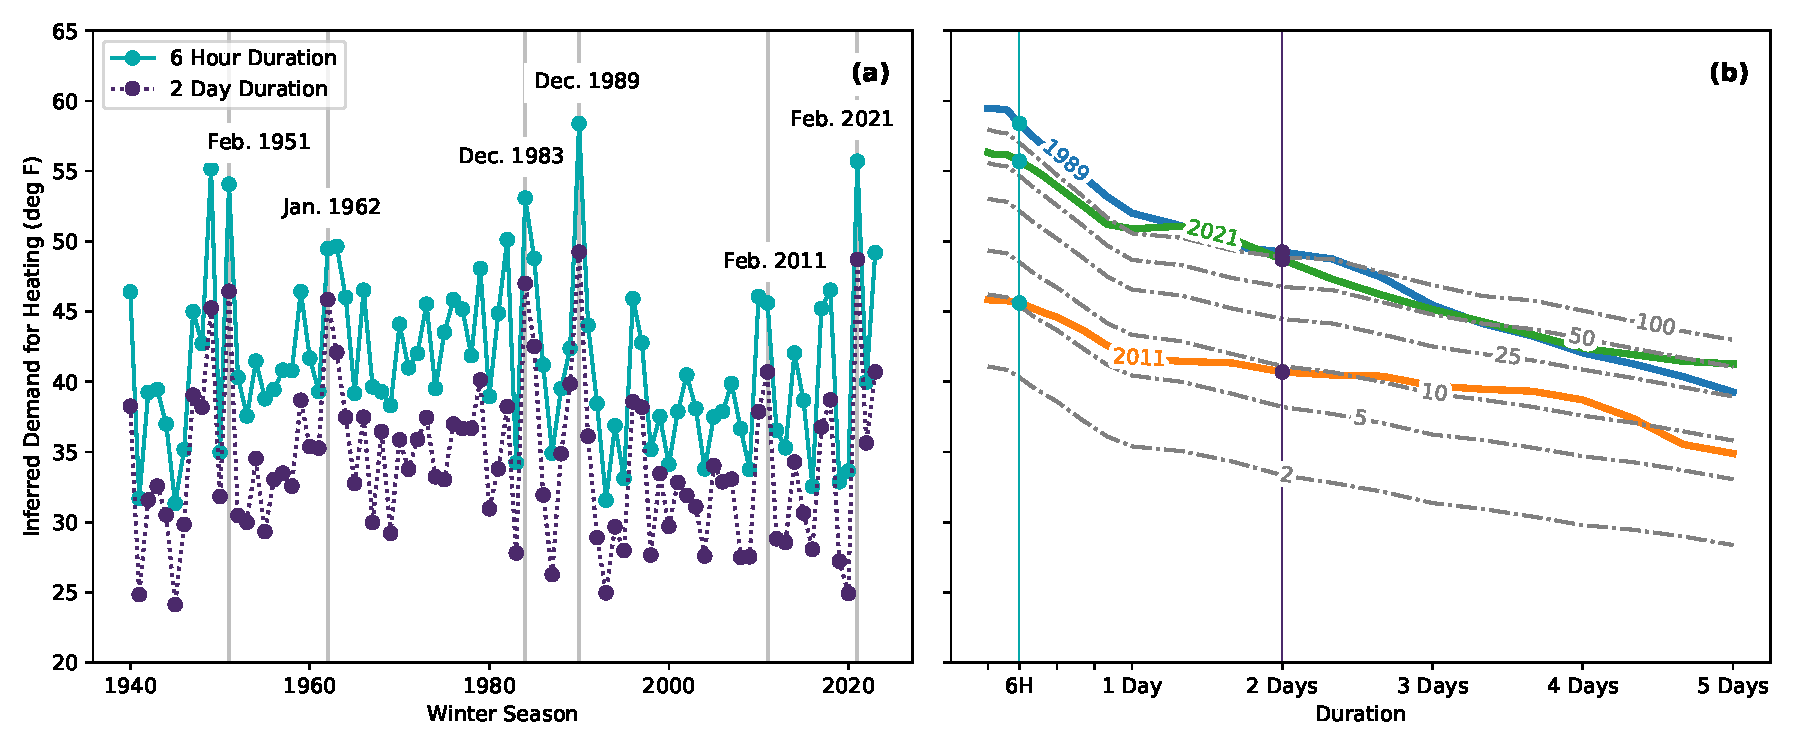
\includegraphics[width=\textwidth]{ERCOT_HDD_IDF_MLE_popweighted.pdf}\\
            \caption{
                \textbf{The \emph{inferred heating demand per capita} induced by the February 2021 cold snap is not unprecedented.}
                (a): time series of annual maximum \emph{inferred heating demand per capita}.
                (b): the intensity-duration-frequency (IDF) intervals, estimated using 1950-2020 data, overlaid by annual maxima from 1989, 2011, and 2021.
                Each dashed line shows a single return level (2, 5, 10, 25, 50, 100 year) for \emph{inferred heating demand per capita} averaged over a given duration ($x$-axis).
                Gray dashed lines indicate 2, 5, 10, 25, 50, and 100 year return levels.
            }\label{fig:idf_weighted}
        \end{figure}
    \end{framed}
\end{block}